%!TEX root =  main.tex
\pagestyle{fancy}
\fancyhf{}
\fancyhead[RE,LO]{\leftmark}
\fancyfoot[CE,CO]{\thepage}
\chapter{Introduction}\label{chapter:Intro}
%
Various software systems has changed the way people communicate, learn and run businesses, and interconnected computing devices has numerous positive applications in everyday life. Over the past decade, computation and data volumes have increased significantly~\cite{ChiangZ16}. Augmented reality, online gaming, face recognition, autonomous vehicles, or the Internet of Things (IoT) applications produce huge volumes of data. Workloads like those require latency below a few tens of milliseconds~\cite{ChiangZ16}. These requirements are outside what a centralized model like the CC can offer~\cite{ChiangZ16}. Even small problems can contribute to large downtime of applications and servies people are depending on. Recent example is yet another outage that happend in Amazon Web Services (AWS), and as a result a large amount of intrnet become unavaleble.

The aim of this thesis is to provide formal models uppon which we implement distributed system for oragnizing cloud-like geo-distributed environments for users or CC providers to utilize, in order to minimize downtime of critical services. The whole system can be looked as a pre-cloud or pre-processing layer sending only important data to the cloud minimizing cost for users, and ensuring avelability of CC services. Ensuring reliability and correctness of any system is very difficult, and should be mathematically based. Formal methods are techniques that allow us specification and verification of complex (software and hardware) systems based on mathematics and formal logic.

We start by describing the general problem area that our work addresses in Section~\ref{sec:problem_area}. Sections~\ref{sec:distributed_systems} and \ref{sec:distributed_computing} describe the theoretical background behind the problem, where we examine distributed systems and distributed computing, focusing on design details, communication patters and organizational structure. In Section~\ref{sec:problem_statement}, we specify the exact problem that our work addresses and describe our hypothesis and research goals in Section~\ref{sec:research_hyphotesis_and_golas}. Section~\ref{sec:structure_of_thesis} present the structure of the thesis.
%
%
%
\section{Problem area}\label{sec:problem_area}
%
Cloud centralized architecture with enormous data-centers (DCs) capacities creates an effective economy of scale to lower administration cost~\cite{BariBEGPRZZ13}. However, when such a  system grows to its limits, centralization brings more problems than solutions~\cite{GunawiHSLSAE16, LopezMEDHIBFR15}. Despite all the CC benefits, applications and services face a serious degradation over time, due to the high bandwidth and latency~\cite{KarimIWGSYO16}. This can have a huge consequence on the business and potentially human lives as well. Organizations use cloud services to avoid huge investments~\cite{MonsalveCC18}, like creating and maintaining their own DCs. They consume resources created by others~\cite{Satyanarayanan17} and pay for usage time -- a pay as you go model.

Data is required to be moved to the cloud from data sources, which introduces a high latency in the system~\cite{HossainRH18}. For example, Boeing 787s generates half a terabyte of data per single flight, while a self-driving car generates two petabytes of data per single drive. Bandwidth is not large enough to support such requirements~\cite{CaoZS18}. Data transfer is not the only problem: applications like self-driving cars, delivery drones, or power balancing in electric grids require real-time processing for proper decision making \cite{CaoZS18}. We might face serious issues if a cloud service becomes unavailable due to denial-of-service attack, network, or cloud failure~\cite{GunawiHSLSAE16}.

To overcome cloud latency, research led to new computing areas, and model in which computing and storage utilities are in proximity to data sources~\cite{Satyanarayanan17}. The cloud is enhanced with new ideas for future generation applications~\cite{NingLSY20}. 
%
%
%
\section{Distributed systems}\label{sec:distributed_systems}
%
There are various definitions of distributed systems (DS), but we can think of DS as a systems where multiple entities can comunicate to one another in some way, but at the same time, they are able to performing some operations. Three significant characteristics of distributed systems are: $(1)$~\textbf{concurrency of components}, $(2)$~\textbf{lack of a global clock}, and $(3)$~\textbf{independent failure of components}~\cite{0019513}. In~\cite{SteenT16} authors give formal definition \say{distributed system is a collection of autonomous computing elements that appears to its users as a single coherent system}.

When talking about DS, we usually think about computing systems that are connected via network or over the internet. But DS are not exclusiv to domain of cumputer science. They existed before computers started to enrich almost every aspect of human life. DS have been used in varios different domains such as: \textbf{telecommunication networks}, \textbf{aircraft control systems}, \textbf{industrial control systems} etc. DS are used anywhere where amout of users are growing rapidly, so that single entity can't reponse to users demands in (near) real-time.

This section will explain different aspects of DS in computing systems, that are important for future pars of the thesis. Section~\ref{sec:scalability} gives more details about scalability and what it meens in modern day computer applications. Section~\ref{sec:cloud_computing} gives explanation what CC is, organizational aspects of CC as well as used models. Section~\ref{sec:p2p_networks} gives explanation what peer-to-peer networks are, and why are they important in modern DS. Section~\ref{sec:mobile_computing} gives general deffinition what mobile computing is and new ways of implementation DS.
%
%
%
\subsection{Scalability}\label{sec:scalability}
%
Scalability is the property of a system to handle a growing amount of work by adding resources to the system~\cite{Bondi00}. When talking about computer systems scalability can be represented in two flavors:

\begin{itemize}
	\item \textbf{Scaling vertically} means upgradeing the hardware that computer systems are running on. Vertical scaling can increase performance to what latest hardware can offer, and here we are limited by the laws of phisics and Moor's law \cite{Gustafson2011}. Tipical example that require this type of scaleing is relation dataase server. These capabilities are insufficient for moderate to big workloads.
	\item \textbf{Scaling horizontally} means that we scale our system by keep adding more and more computers, rather than upgrading the hardware of a single one. With this apporouch we are (almost) limitless how much we can scale. Whenever performance degrades we can simply add more computers (or nodes). These nodes are not required to be some high-end machines.
\end{itemize}

Table~\ref{tab:table1} summarize differences between horizontall and verticall scaling.

\begin{table}[h!]
	\begin{center}
		\begin{tabular}{l|l|l}
			  & \textbf{Scaling vertically} & \textbf{Scaling horizontally}\\
			\hline
			\textbf{Scaling} & Limited & Unlimited \\
			\textbf{Managment} & Easy & Comlex\\
			\textbf{Investments} & Expensive & Afordable \\
		\end{tabular}
	\end{center}
	\vspace{-0.5cm}
	\caption{Differences between horizontall and verticall scaling.}
	\label{tab:table1}
\end{table}

Scaling horizontally is a preferable way for scaling DS, not because we can scale easier, or because it is significantly cheaper than vertical scaling after a certain threshold~\cite{Bondi00} but because this approuch comes with few more benefits that are esspecially important when talking large-scale DS. Adding more nodes gives us two important properties: 

\begin{itemize}
	\item \textbf{Fault tolerance} means that applications running on multiple places at the same time, are not bound to the fail of node, cluster or even data center (DC). As long as there is a copy of application running somewhere, user will get response back. This means that service is more \textbf{avalible}, that running on a single node no metter how high-end that node is. Eventually all nodes are going to break.
	\item \textbf{Low latency} refers to the idea that the world is limited by the speed of light. If a node running application is too far away, user will wait too long for the response to get back. If same application is running on multiple places, user request will hit node that is closest to the user.
\end{itemize}

But despite all the obvious benefits, for a DS to work properly, we need the write software in such a way that is able to run on multiple nodes, as well as that accept \textbf{failure} and deal with it. This turns out to be not an easy task.
%
%
\subsection{Cloud computing}\label{sec:cloud_computing}
%
We can define cloud computing (CC) like aggregation of computing resources as a utility, and software as a service~\cite{Vogels}. Hardware and software in big DC provide services for user consumption over the internet~\cite{AboveTheCloud}. Resources like CPU, GPU, storage, and network are utilities and can be used as well as released on-demand~\cite{ZhangCB10}. The key strength of the CC are offered services~\cite{Vogels}. 

The traditional CC model provides enormous computing and storage resources elastically, to support the various applications needs. This property refers to the cloud ability to allow services, allocation of additional resources, or release unused ones to match the application workloads on-demand~\cite{AssuncaoVB18}. Services usually fall in one of three main categories: 
\begin{itemize}
	\item \textbf{Infrastructure as a service (IaaS)} allows businesses to purchase resources on-demand and as-needed instead of bying and manageing hardware themself.
	\item \textbf{Platform as a service (PaaS)} delivers a framework for developers to create, maintain and manage their applications. All resources are managed by the enterprise or a third-party vendor.
	\item \textbf{Software as a service (SaaS)} deliver applications over the internet to its users. These applications are managed by a third-party vendor, .
\end{itemize}

Figure~\ref{fig:fig1} show difference in control and management of resources between different cloud options and on-premises solution.

\begin{figure}[H]
	\begin{center}
		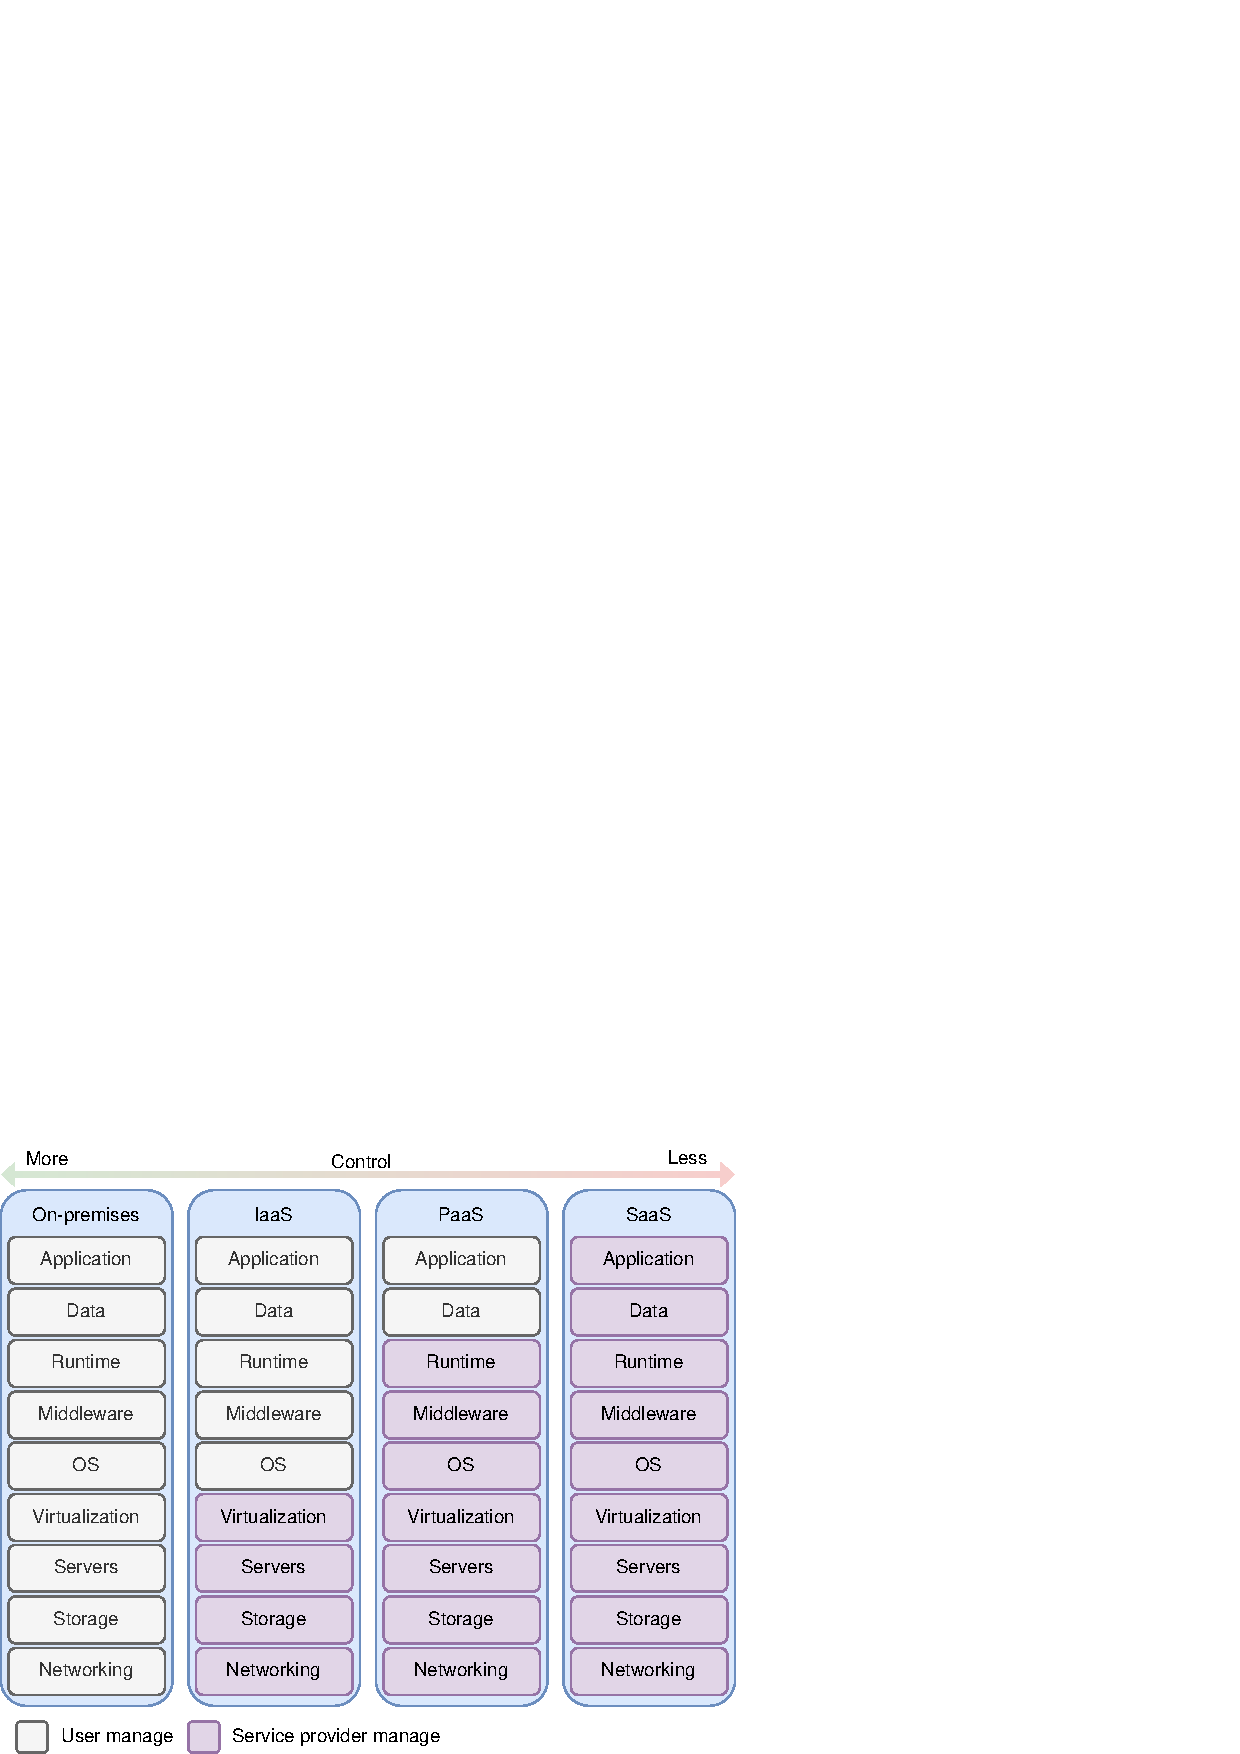
\includegraphics[scale=0.9]{images/Figure1.png}
	\end{center}
	\vspace{-0.6cm}
	\caption{Difference between cloud options and on-premises solution.}
	\label{fig:fig1}
\end{figure}

The user can choose a single solution, or combine more of them if such a thing is required depending on preferences and needs.

CC has been the dominating tool in the past decade in various applications~\cite{Satyanarayanan17}. It is changing, evolving, and offering new types of services. Resources such as container as a service (CaaS), database as a service (DBaaS)~\cite{Peter} are newly introduced. The CC model gives us a few benefits. Centralization relies on the economy of scale to lower the cost of administration of big DC. Organizations using cloud services avoid huge investments. Like creating and maintaining their own DC. They consume resources created by others~\cite{Satyanarayanan17} and pay for usage time -- a pay as you go model. 

Over the years there are more as a service options avalible, forming \textbf{everything as a service (XaaS)} model~\cite{DuanFZSNH15}. This model propose that any hardware or software resource can be ofered as a service to the users over the internet.

Table~\ref{tab:table2} shows common examples of SaaS, PaaS, and IaaS applications.

\begin{table}[h!]
	\begin{center}
		\begin{tabular}{l|l}
			\textbf{Platform type} & \textbf{Common Examples}\\
			\hline
			\textbf{IaaS} & AWS, Microsoft Azure, Google Compute Engine \\
			\textbf{PaaS} & AWS Elastic Beanstalk, Azure, App Engine \\
			\textbf{SaaS} & Gmail, Dropbox, Salesforce, GoToMeeting \\
		\end{tabular}
	\end{center}
	\vspace{-0.5cm}
	\caption{common examples of SaaS, PaaS, and IaaS.}
	\label{tab:table2}
\end{table}

CC is giving a user an illusion that he is using single machine, while the backgroud implementaion is fairly complicated and consists of various elements that are composed of countles machines. CC is tipical example of horizontally scalable system explained in~\ref{sec:scalability}
%
%
\subsection{Peer-to-peer networks}\label{sec:p2p_networks}
%
Peer-to-peer (P2P) communication is a networking architecture model that partitions tasks or workloads between peers~\cite{Schollmeier01}. All peers are created equally in the system, and there is no such thing as a node that is more important then others. Every Peer have a portion system resources, such as processing power, disk storage or network bandwidth, directly available to other network participants, without the need for central coordination by servers or stable hosts~\cite{Schollmeier01}. P2P nodes are connected and share resources without going through a separate server computer that is responsabile for routing. Figure~\ref{fig:fig2} show difference in network topology between P2P networks $(a)$ and client-server architecture $(b)$.

\begin{figure}[H]
	\begin{center}
		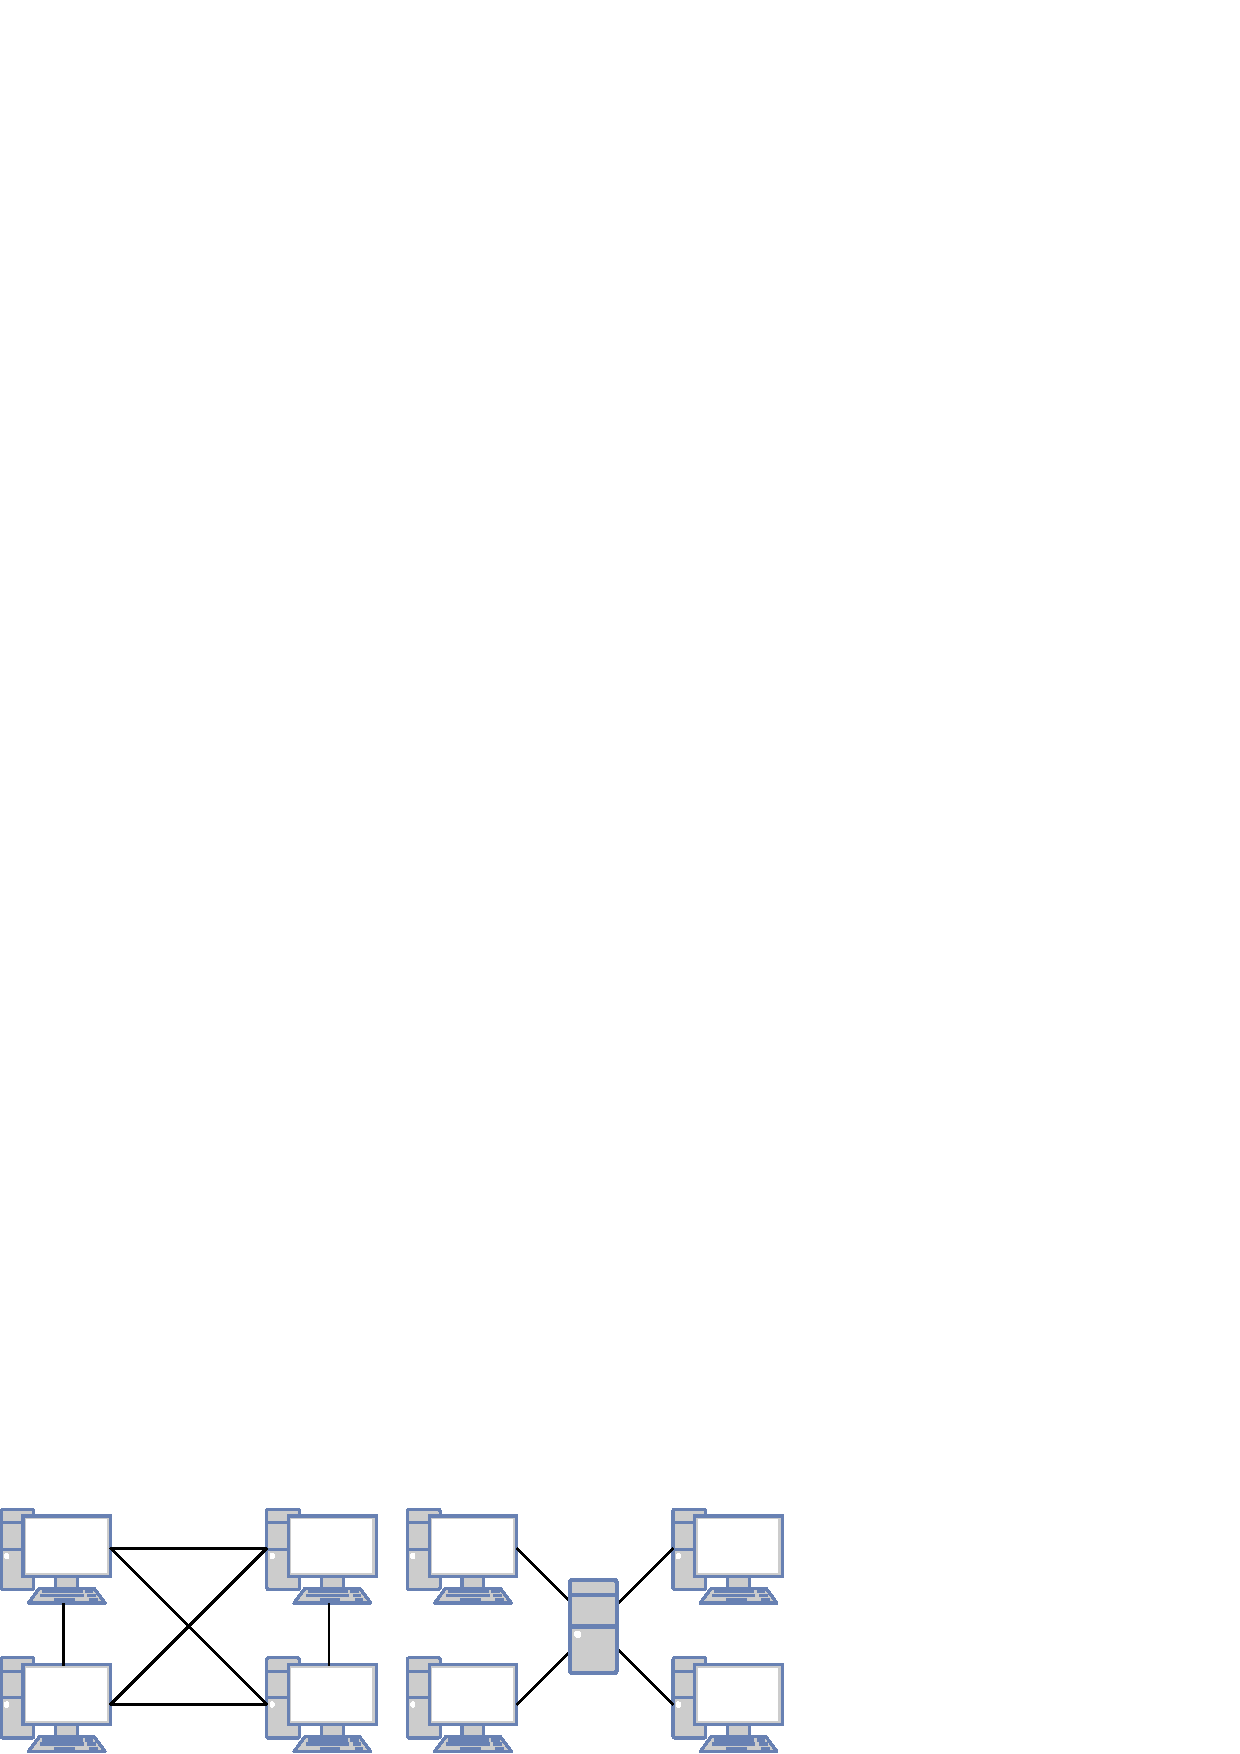
\includegraphics[scale=0.7]{images/Figure2.png}
	\end{center}
	\vspace{-0.6cm}
	\caption{$(a)$ P2P network and $(b)$ client-server network.}
	\label{fig:fig2}
\end{figure}

Peers are creating a sense of virtual community. This community of peers can resolve a greater tasks, beyond those that individual peers can do. Yet, these tasks are beneficial to all the peers in the system~\cite{BandaraJ13}.

Based on how the nodes are linked to each other within the overlay network, and how resources are indexed and located, we can classify networks as~\cite{KamelSE07}:
\begin{itemize}
	\item \textbf{Unstructured} do not have a particular structure by design, but they are formed by nodes that randomly form connections~\cite{FilaliBHB11}. Their strenght and weaknes at the same time is ther lack of structure. These networks and robust when peers join and leave network. But when doing query, they must found more possible peers that have same peace of data. Tipical example of this group is a Gossip-based protocols like~\cite{DasGM02}.
	\item \textbf{Structured} peers are organized into a specific topology, and the protocol ensures that any node can efficiently search the network for a resource. The famos type of structured P2P network is a Distributed Hash Table (DHT). These networks maintain lists of neighbors to do more efficent lookup, and as such they are not so robust when nodes join or leave the network. DHT commonly used in resource loopkup systems~\cite{StoicaMKKB01}, and as efficent resource lookip management and scheduling of applications, or as an integral part of distributed storage systems and NoSQL\cite{Leavitt10} databases.
	\item \textbf{Hybrid} combine previous two models in various ways.
\end{itemize}

P2P networks are great tool in many arsenals, but because their unique ability to act as a server and as a client at the same time we must be aware and pay more attention to security because they are more vulnerable to exploits~\cite{0024003}/
%
%
\subsection{Mobile computing}\label{sec:mobile_computing}
%
Mobile cloud computing (MCC), was the first idea that introduced task offloading~\cite{FernandoLR13, LinLJL19}. Heavy computation remains in the cloud. Mobile devices run small client software and interact with the cloud, over the internet using his resources. 

The main problem with MCC is that the cloud is usually far away from end devices. That leads to high latency and bad quality of experience (QoE)~\cite{LinLJL19}. Especially for latency-sensitive applications. Even though MCC is not that much different from the standard cloud model. We had moved a small number of tasks from the cloud. Thus opening the door for future models.

To overcome cloud latency and MCC problems, research led to new computing areas like edge computing (EC). EC is a model in which computing and storage utilities are in proximity to data sources~\cite{Satyanarayanan17}. The cloud is enhanced with new ideas for future generation applications~\cite{NingLSY20}. 

Over the years, designs like fog~\cite{BonomiMNZ14}, cloudlets~\cite{MonsalveCC18}, and mobile edge computing (MEC)~\cite{WangZZWYW17} emerged. In this thesis, we refer to all these models as edge nodes. They all use the concept of data and computation offloading from the cloud closer to the ground~\cite{KhuneP19}, while heavy computation remains in the cloud because of resource availability~\cite{NingLSY20}. 

EC models introduce small-scale servers that operate between data sources and the cloud. Typically, they have much less capabilities compared to the cloud counterparts~\cite{ChenHLLW15}. These servers can be spread in base stations~\cite{WangZZWYW17}, coffee shops, or over geographic regions to avoid latency as well as huge bandwidth~\cite{MonsalveCC18}. They can serve as firewalls~\cite{SatyanarayananK19} and pre-processing tier, while users get a unique ability to dynamically and selectively control the information sent to the cloud.


\section{Distributed computing}\label{sec:distributed_computing}
%
%
\subsection{Big Data}\label{sec:big_data}
%
%
\subsection{Microservices}\label{sec:microservices}
%
%


\subsection{Parallel computing}\label{sec:parallel_computing}
%
%


\section{Problem Statement}\label{sec:problem_statement}
%
%



\section{Research Hypotheses, and Goalst}\label{sec:research_hyphotesis_and_golas}
%
%




\section{Structure of the thesis}\label{sec:structure_of_thesis}
%
%


